\begin{exercises} 

\item Find the indicated derivative.  In each case, state the version of the Chain Rule that you are using.
	\ba	
	\item $\frac{df}{dt}$, if $f(x,y) = 2x^2y$, $x=\cos(t)$, and $y=\ln(t)$.

	\item $\frac{\partial f}{\partial w}$, if $f(x,y) = 2x^2y$, $x=w+z^2$, and $y=\frac{2z+1}{w}$



	\item $\frac{\partial f}{\partial v}$, if $f(x,y,z) = 2x^2y+z^3$, $x=u-v+2w$, $y=w2^v-u^3$, and $z = u^2-v$
	\ea

\begin{exerciseSolution}
\ba 
\item The chain rule says that
\begin{align*}
\frac{df}{dt} &= \frac{\partial f}{\partial x}\frac{dx}{dt} + \frac{\partial f}{\partial y}\frac{dy}{dt} \\
	&= (4xy)\left(-\sin(t)\right) + (2x^2)\left(\frac{1}{t}\right) \\
	&= -4 \cos(t) \sin(t) \ln(t) + \frac{2\cos^2(t)}{t}.
\end{align*}
\item By the chain rule we have
\begin{align*}
\frac{\partial f}{\partial w} &= \frac{\partial f}{\partial x} \frac{\partial x}{\partial w}+ \frac{\partial f}{\partial y} \frac{\partial y}{\partial w} \\
	&= \left( 4xy \right)\left( 1 \right) + \left( 2x^2 \right)\left( -\frac{2z+1}{w^2} \right) \\
	&= \left( \frac{(2z+1)4(w+z^2)y}{w} \right) - \left( \frac{2(2z+1)((w+z^2)^2}{w^2} \right).
\end{align*}

\item By the chain rule we have
\begin{align*}
\frac{\partial f}{\partial v} &= \frac{\partial f}{\partial x} \frac{\partial x}{\partial v}+ \frac{\partial f}{\partial y} \frac{\partial y}{\partial v} + \frac{\partial f}{\partial z} \frac{\partial z}{\partial v} \\
	&= \left( 4xy \right)\left( -1 \right) + \left( 2x^2 \right)\left( w^2 \right) + \left( 3z^2 \right)\left( -1 \right)  \\
	&= -4(u-v+2w)(w2^v-u^3) + 2(u-v+2w)^2w^2 - 3(u-v+2w)^2.
\end{align*}

\ea

\end{exerciseSolution}

\item Let $z = u^2 - v^2$ and suppose that
    \begin{align*}
      u & = e^x\cos y \\
      v & = e^x\sin y
    \end{align*}
    
    \ba
      \item Find the values of $u$ and $v$ that correspond to $x=0$ and $y=2\pi/3$.
      \item Use the Chain Rule to find the general partial derivatives
        $$
        \frac{\partial z}{\partial x}
        \hspace*{20pt}
        \mbox{and}
        \hspace*{20pt}
        \frac{\partial z}{\partial y}
        $$
        and then determine both $\frac{\partial z}{\partial x}\bigm|_{(0, \frac{2\pi}{3})}$ and $\frac{\partial z}{\partial y}\bigm|_{(0, \frac{2\pi}{3})}$.
     \ea

\begin{exerciseSolution}
    \ba
      \item Evaluating $u$ and $v$ at $x=0$ and $y=2\pi/3$ yields
\[u(0,2\pi/3) = \cos(2\pi/3) = -\frac{1}{2} \ \text{ and } \ v(0,2\pi/3) = \sin(2\pi/3) = \frac{\sqrt{3}}{2}.\]
      \item By the Chain Rule we have
\begin{align*}
\frac{\partial z}{\partial x} &= \frac{\partial z}{\partial u} \frac{\partial u}{\partial x} + \frac{\partial z}{\partial v} \frac{\partial v}{\partial x} \\
	&= 2ue^x\cos(y) -2ve^x \sin(y) \\
	&= 2e^{2x}\cos^2(y) - 2e^{2x}\sin^2(y)
\end{align*}
and
\begin{align*}
\frac{\partial z}{\partial y} &= \frac{\partial z}{\partial u} \frac{\partial u}{\partial y} + \frac{\partial z}{\partial v} \frac{\partial v}{\partial y} \\
	&= -2ue^x\sin(y) -2ve^x \cos(y) \\
	&= -2e^{2x}\cos(y)\sin(y) - 2e^{2x}\sin(y)\cos(y) \\
	&= -4e^{2x}\cos(y) \sin(y).
\end{align*}
Note that 
\[\frac{\partial z}{\partial x} = 2u^2-2v^2 \ \text{ and } \ \frac{\partial z}{\partial y} = -4uv,\]
so
\begin{align*}
\frac{\partial z}{\partial x}\biggm|_{(0, \frac{2\pi}{3})} &= 2\left(-\frac{1}{2}\right)^2 -2\left(\frac{\sqrt{3}}{2}\right)^2 = -1 \\
\frac{\partial z}{\partial y}\biggm|_{(0, \frac{2\pi}{3})} &= -4\left(-\frac{1}{2}\right)\left(\frac{\sqrt{3}}{2}\right) = \frac{2\sqrt{3}}{2}.
\end{align*}
     \ea
\end{exerciseSolution}
        
 \item Suppose that $T = x^2 + y^2 - 2z$ where
  \begin{align*}
    x & = \rho\sin\phi\cos\theta \\
    y & = \rho\sin\phi\sin\theta \\
    z & = \rho\cos\phi
  \end{align*}

  \ba
    \item Construct a tree diagram representing the dependencies among the variables.
    \item Apply the chain rule to find the partial derivatives
      $$
      \frac{\partial T}{\partial\rho},
      \frac{\partial T}{\partial\phi},
      \ 
      \mbox{and}
      \ 
      \frac{\partial T}{\partial\theta}.
      \hspace*{20pt}
      $$
    \ea

\begin{exerciseSolution}

  \ba
    \item A tree diagram that represents the dependencies among the variables is shown below.
\begin{center}
\setlength{\unitlength}{1.0cm}
\begin{picture}(7,5)
\put(0,0){$\rho$}
\put(1,0){$\phi$}
\put(2,0){$\theta$}

\put(2.5,0){$\rho$}
\put(3.5,0){$\phi$}
\put(4.5,0){$\theta$}

\put(5,0){$\rho$}
\put(6,0){$\phi$}
\put(7,0){$\theta$}

\put(1,2){$x$}
\put(3.5,2){$y$}
\put(6,2){$z$}

\put(3.5,4){$T$}

\put(0.2,0.35){\line(1,2){0.75}}
\put(1.1,0.35){\line(0,1){1.5}}
\put(2.0,0.35){\line(-1,2){0.75}}

\put(2.7,0.35){\line(1,2){0.75}}
\put(3.6,0.35){\line(0,1){1.5}}
\put(4.5,0.35){\line(-1,2){0.75}}

\put(5.2,0.35){\line(1,2){0.75}}
\put(6.1,0.35){\line(0,1){1.5}}
\put(7.0,0.35){\line(-1,2){0.75}}

\put(1.4,2.2){\line(5,4){2.0}}
\put(3.6,2.3){\line(0,1){1.5}}
\put(5.9,2.2){\line(-5,4){2.0}}
\end{picture}
\end{center}.

    \item By the Chain Rule we have 
\begin{align*}
\frac{\partial T}{\partial\rho} &= \frac{\partial T}{\partial x} \frac{\partial x}{\partial\rho} + \frac{\partial T}{\partial y} \frac{\partial y}{\partial\rho}  + \frac{\partial T}{\partial z} \frac{\partial z}{\partial\rho} \\
	&= 2x\sin(\phi) \cos(\theta) + 2y\sin(\phi) \sin(\theta) - 2\cos(\phi) \\
	&= 2\rho\sin^2(\phi) \cos^2(\theta) + 2\rho\sin^2(\phi) \sin^2(\theta) - 2\rho\cos^(\phi),
\end{align*}
\begin{align*}
\frac{\partial T}{\partial \phi} &= \frac{\partial T}{\partial x} \frac{\partial x}{\partial \phi} + \frac{\partial T}{\partial y} \frac{\partial y}{\partial \phi}  + \frac{\partial T}{\partial z} \frac{\partial z}{\partial \phi} \\
	&= 2x \rho \cos(\phi) \cos(\theta) + 2y \rho \cos(\phi) \sin(\theta) + 2\sin(\phi) \\
	&= 2\rho^2 \cos(\phi) \sin(\phi) \cos^2(\theta) + 2\rho^2 \cos(\phi) \sin(\phi) \sin^2(\theta) + 2\sin^(\phi),
\end{align*}
and
\begin{align*}
\frac{\partial T}{\partial \theta} &= \frac{\partial T}{\partial x} \frac{\partial x}{\partial \theta} + \frac{\partial T}{\partial y} \frac{\partial y}{\partial \theta}  + \frac{\partial T}{\partial z} \frac{\partial z}{\partial \theta} \\
	&= -2x \rho \sin(\phi) \sin(\theta) + 2y \rho \sin(\phi) \cos(\theta)  \\
	&= -2\rho^2 \sin^2(\phi) \cos(\theta) \sin(\theta) + 2\rho^2 \sin^2(\phi) \cos(\theta) \sin(\theta).
\end{align*}

    \ea
    

\end{exerciseSolution}
     
\item Suppose that the temperature on a metal plate is given by
    the function $T$ with 
    $$
    T(x,y) = 100-(x^2 + 4y^2),
    $$
    where the temperature is measured in degrees Fahrenheit
    and $x$ and $y$ are each measured in feet. 
    Now suppose that an ant is walking on the metal plate in such a way that it walks in a straight line from the point $(1,4)$ to the point $(5,6)$.
    \ba
    	\item Find parametric equations $(x(t),y(t))$ for the ant's coordinates as it walks the line from $(1,4)$ to $(5,6)$.
	\item What can you say about $\frac{dx}{dt}$ and $\frac{dy}{dt}$ for every value of $t$?
	\item Determine the instantaneous rate of change in temperature with respect to $t$ that the ant is experiencing at the moment it is halfway from $(1,4)$ to $(5,6)$, using your parametric equations for $x$ and $y$.  Include units on your answer.
    \ea    

\begin{exerciseSolution}
    \ba
    \item A direction vector for this line is $\langle 5-1, 6-4 \rangle = \langle 4, 2 \rangle$, so parametric equations $(x(t),y(t))$ for the ant's coordinates as it walks the line from $(1,4)$ to $(5,6)$ are
\[x(t) = 1 + 4t \ \text{ and } \ y(t) = 4 + 2t.\]

	\item Since $x$ and $y$ are linear functions of $t$, we see that $\frac{dx}{dt} = 4$ and $\frac{dy}{dt} = 2$ are both constant. 
	
	\item We want $\frac{dT}{dt}\bigm|_{t=1/2}$. The Chain Rule tells us that 
	\begin{align*}
	\frac{dT}{dt} &= \frac{\partial T}{\partial x} \frac{dx}{dt} + \frac{\partial T}{\partial y} \frac{dy}{dt} \\
		&= (-2x)(4) + (-8y)(2) \\
		&= -8(1 + 4t) - 16(4 + 2t).
	\end{align*}
	So
	\[\frac{dT}{dt}\biggm|_{t=1/2} = -8(3) - 16(5) = 104 \ \frac{^{\circ}\text{F}}{\text{ft}}.\]
		
    \ea  
\end{exerciseSolution}
     
\item There are several proposed formulas to approximate the surface
   area of the human body.
   One model\footnote{DuBois D, DuBois DF. A formula to
     estimate the approximate surface area if height and weight be
     known.  \emph{Arch Int Med} 1916;17:863-71.} uses the formula
   $$
    A(h,w) = 0.0072 h^{0.725}w^{0.425},
   $$
   where $A$ is the surface area in square meters, $h$ is the
   height in centimeters, and $w$ is the weight in kilograms.

   Since a person's height $h$ and weight $w$ change over time,
  $h$ and $w$ are functions of time
   $t$. Let us think about what is happening to a child whose height
  is $60$ centimeters and weight is $9$ kilograms. Suppose,
  furthermore, that 
  $h$ is increasing at an instantaneous rate of 20 centimeters per year and $w$ is
 increasing at an instantaneous rate of $5$ kg per year. 

 Determine the instantaneous rate at which the child's surface area is changing at this point in time.

\begin{exerciseSolution}
We want to find $\frac{dA}{dt}\bigm|_{(60,9)}$ given that $\frac{dh}{dt} = 20$ and $\frac{dw}{dt} = 5$. The Chain Rule tells us that 
\begin{align*}
\frac{dA}{dt} &= \frac{\partial A}{\partial h} \frac{dh}{dt} + \frac{\partial A}{\partial w} \frac{dw}{dt} \\
	&= 0.00522h^{-0.275}w^{0.425}(20) + 0.00306h^{0.725}w^{-0.575}(5).
\end{align*}
So
\[\frac{dA}{dt}\biggm|_{(60,9)} \approx 0.1703 \ \frac{\text{m}^2}{\text{yr}}.\]
\end{exerciseSolution}

\item Let $z = f(x,y) = 50 - (x+1)^2 - (y+3)^2$ and $z = h(x,y) = 24 - 2x - 6y$.

Suppose a person is walking on the surface $z = f(x,y)$ in such a way that she walks the curve which is the intersection of $f$ and $h$. 
	\ba
	\item Show that $x(t) = 4 \cos(t)$ and $y(t) = 4 \sin(t)$ is a parameterization of the ``shadow'' in the $x$-$y$ plane of the curve that is the intersection of the graphs of $f$ and $h$.

	\item Use the parameterization from part (a) to find the instantaneous rate at which her height is changing with respect to time at the instant $t = 2\pi/3$.  
	
	\ea

\begin{exerciseSolution}
	\ba
	\item Notice that $f(x,y) = h(x,y)$ when $50-x^2-2x-1-y^2-6y-9=24-2x-6y$ or when $x^2+y^2=16$. This is the circle centered at the origin of radius 4, which has a parameterization $x(t) = 4 \cos(t)$ and $y(t) = 4 \sin(t)$.  

	\item We want to find $\frac{df}{dt}\bigm|_{t=2\pi/3}$. The Chain Rule tells us that 
\begin{align*}
\frac{df}{dt} &= \frac{\partial f}{\partial x} \frac{dx}{dt} + \frac{\partial f}{\partial y} \frac{dy}{dt} \\
	&= (-2(x+1))(-4\sin(t)) + (-3(y+3)^2)(4\cos(t)).
\end{align*}
Now $x(2\pi/3) = -2$ and $y(2\pi/3) = 2\sqrt{3}$, so 
\[\frac{df}{dt}\biggm|_{t=2\pi/3} \approx 243.78.\]

	\ea

\end{exerciseSolution}

\item The voltage $V$ (in volts) across a circuit is given by Ohm's Law: $V = IR$, where $I$ is the current (in amps) in the circuit and $R$ is the resistance (in ohms). Suppose we connect two resistors with resistances $R_1$ and $R_2$ in parallel as shown in Figure \ref{F:10.5.CR_Circuit}. The total resistance $R$ in the circuit is then given by
\[\frac{1}{R} = \frac{1}{R_1} + \frac{1}{R_2}.\]
\begin{figure}[ht]
\begin{minipage}{4in}
        \ba
    \item Assume that the current, $I$, and the resistances, $R_1$ and $R_2$, are changing over time, $t$. Use the Chain Rule to write a formula for $\frac{dV}{dt}$.



    \item Suppose that, at some particular point in time, we measure the current to be 3 amps and that the current is increasing at $\frac{1}{10}$ amps per second, while resistance $R_1$ is 2 ohms and decreasing at the rate of 0.2 ohms per second and $R_2$ is 1 ohm and increasing at the rate of $0.5$ ohms per second. At what rate is the voltage changing at this point in time?



    \ea
\end{minipage} \hspace{0.2in}
\begin{minipage}{2.3in}
\begin{center}
%\resizebox{!}{1.15in}{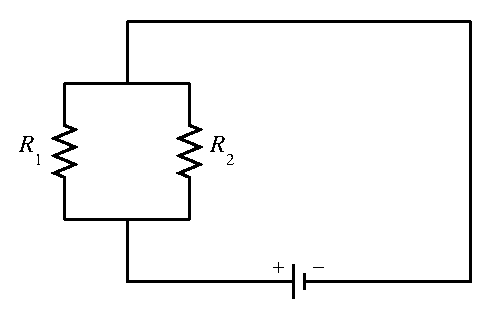
\includegraphics{10_5_CR_Circuit}}
 \includegraphics{figures/fig_10_5_resistors.eps}
\end{center}
\caption{Resistors in parallel.}
\label{F:10.5.CR_Circuit}
\end{minipage}
\end{figure}

\begin{exerciseSolution}
        \ba
    \item Given that $R = \frac{R_1R_2}{R_1+R_2}$ we have 
\[V(I,R_1,R_2) = \frac{IR_1R_2}{R_1+R_2}.\]
The Chain Rule tells us that 
\begin{align*}
\frac{dV}{dt} &= \frac{\partial V}{\partial I} \frac{dI}{dt} + \frac{\partial V}{\partial R_1} \frac{dR_1}{dt} + \frac{\partial V}{\partial R_2} \frac{dR_2}{dt} \\
	&=  \left(\frac{R_1R_2}{R_1+R_2}\right)\frac{dI}{dt} + \left(\frac{IR_2^2}{(R_1+R_2)^2}\right) \frac{dR_1}{dt} +  \left(\frac{IR_1^2}{(R_1+R_2)^2}\right) \frac{dR_2}{dt}.
\end{align*}


    \item Let $t_0$ be this time, then 
\[\frac{dV}{dt}\biggm|_{t=t_0} = \left(\frac{2}{3}\right)(0.1) + \left(\frac{1}{3}\right)(-0.2) + \left(\frac{4}{3}\right)(0.5) = \frac{2}{3} \ \frac{\text{V}}{\text{sec}}.\]




    \ea
\end{exerciseSolution}

\end{exercises}
\afterexercises
